\documentclass[10pt,letterpaper]{article}
\usepackage{multicol}
\usepackage[utf8]{inputenc}
\usepackage{amsmath}
\usepackage{lipsum}
\usepackage{amsfonts}
\usepackage{amssymb}
\usepackage{graphicx}
\usepackage[margin=1in]{geometry}
\graphicspath{{../results/images/}}
\begin{document}
\begin{center}
\begin{huge}
Comparing the Parallel Scalability of Bucketsort, Samplesort, and Bitonic Mergesort.\\
\end{huge}
\vspace{0.25in}
\begin{large}
Coen Valk, Bradford Stone\\
valkc@rpi.edu, stoneb2@rpi.edu\\
\end{large}
\end{center}
\vspace{0.25in}
\begin{multicols}{2}
\begin{abstract}
One of the most primitive and vital operations possible on arrays is sorting. Not only is sorting important for data organization, it is a prerequisite for many more complex array operations. Therefore, it is vital that any sorting algorithm used often is extremely efficient, and able to use available resources as well as possible. In this paper, we test the strong scalability of three different parallel sorting algorithms on an IBM Blue Gene Q system. Furthermore, we test the performance of each algorithm as the size of the array increases and present results for the quickest algorithm in each situation.
\end{abstract}
\section{Introduction}
As the size of input arrays into a sorting algorithm grows, as does the execution time. In serial sorting algorithms, only one comparison is made at a time, while the rest of the array sits idle. Parallel sorting algorithms unlock a new potential to compare multiple parts of the array at the same time, then merging the results to create a full sorted array. High performance computing gives users the ability to greatly speedup execution time by parallelizing the sorting algorithm.

Both members of this project worked together to implement the three sorting algorithms, run the algorithms on the Blue Gene Q system and compile all results.
\section{Analysis}
\subsection{Setup}
Each sorting algorithm was implemented to sort an array of integers given to the root rank. Each array is initialized as a list of random positive integers. The experiment was repeated with array sizes from $2^{20}$ elements up to $2^{25}$ elements, with all powers of two in between tested as well. For each array size, each sorting algorithm was run in parallel from 2 ranks up to 4096 ranks. Each experiment was run on the RPI Blue Gene Q high performance computer. The wall clock execution time for each run was recorded, and the results were compiled to show the strong scaling properties of each algorithm.
\subsection{Bucketsort}

The most interesting attribute of bucketsort is that elements are not pairwise compared. Instead, based on certain attributes they are separated into buckets. In this example, each bucket is an MPI rank. The root sends elements to the proper mpi rank bucket based on the remainder when divided by the number of ranks. then the results are all gathered. The process repeats, putting elements in buckets based on the next series of bits. Eventually this will lead to a sorted sequence of numbers.

With randomly distributed arrays of integers, bucketsort can effectively organize large arrays quickly. However, with many duplicate numbers, or gaussian distributions with a small standard deviation, certain buckets may be much larger than others causing imbalanced load between processes. Imbalance in workload per process may cause significant slowdown due to available resources not being effectively used.

\subsection{Samplesort}

Samplesort is an effective sorting algorithm, similar to bucketsort, where each element is fit into buckets based on it relative size in the array. Different from bucketsort, however, is the clever choosing of pivots from a samples of the array to better balance load between all processes
\cite{samplesort}. Samplesort splits the array into equal parts given to each MPI Rank. Each MPI Rank serially sorts the smaller array. From the sorted arrays, regularly spaced out samples are gathered to the root and merged to make an array of samples. The root selects n pivots, where n is the number of MPI ranks, regularly spaced out from the sample array. This information is scattered to each rank. Following this, each rank determines which other rank to send data to, based on the pivots. Each rank gathers data from all other ranks which fit within its pivot window. 

Because samplesort takes care to pick samples that will balance workload evenly across ranks, Samplesort will most likely show a consistent runtime for different distributions of elements as well such as almost sorted, completely backwards, or Gaussian distribution.

\subsection{Bitonic Mergesort}

Bitonic mergesort, otherwise known as batcher sort odd-even mergesort takes advantage of bitonic sequences to sort an array of numbers \cite{bitonic}. Bitonic arrays contain only one local maximum and one local minimum. Bitonic mergesort merges multiple bitonic sequences into one larger bitonic list, until the entire list can be merged in ascending order. Serially, bitonic mergesort is not as efficient as it could be, due to the constant shuffling and reshuffling into different sized bitonic sequences. However, when executed in parallel, every rank can contribute to creating a bitonic sequence. Therefore, there will most likely be a significant speedup when set in parallel compared to a serial version of bitonic sort.

One particular quirk of Bitonic Mergesort is that the size of the array must be a power of two, due to the process of merging bitonic sequences. This was accounted for in this experiment, but it is possible that this may restrict use for this sorting algorithm in the real world.

\section{Resuts}

After all of the results are compiled, a graph depicting the scalability of each sorting algorithm was created. Bucketsort, while the wall clock time is slower than the other two algorithms, showed significant speedup as the number of available processes increases. The following graph shows the execution time of sorting $2^{20}$ numbers with our bucketsort implementation as the number of processes varies.

\begin{center}
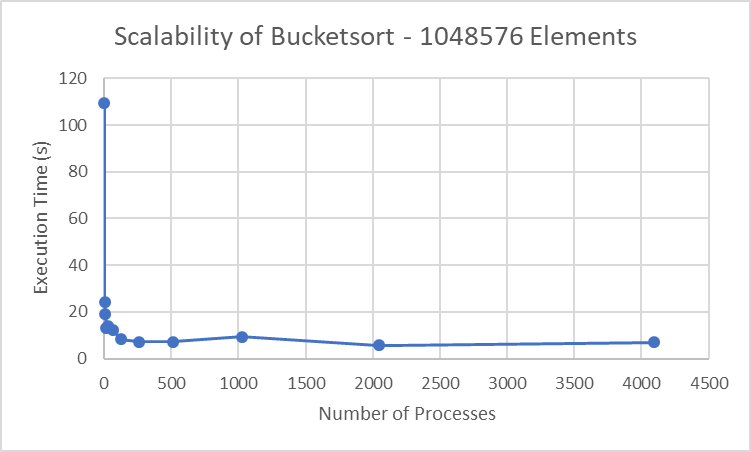
\includegraphics[scale=1]{bucketsort_1048576}
\end{center}

Bitonic mergesort in particular shows impressive scalability. At the largest number of elements, bitonic sort was clearly the fastest algorithm, with an execution time of less than half a second to sort $2^{25}$ elements. Validating our suspicions, at a low number of processors, bitonic sort performs slower than samplesort, but quickly catches up and improves upon samplesort's scalability as the number of processes increases. The following graph demonstrates the execution time of sorting $2^{25}$ elements based on the number of processors, as well as the log graph to more accurately demonstrate the change in execution time as the amount of ranks increases.

\begin{center}
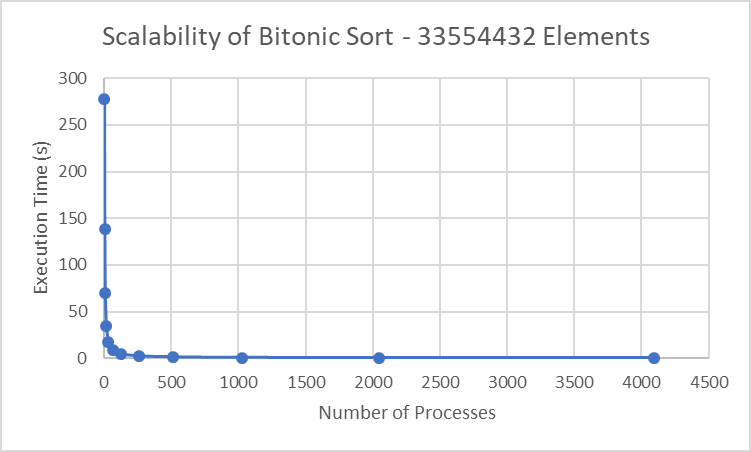
\includegraphics[scale=1]{bitonicsort_33554432}
\end{center}

\begin{center}
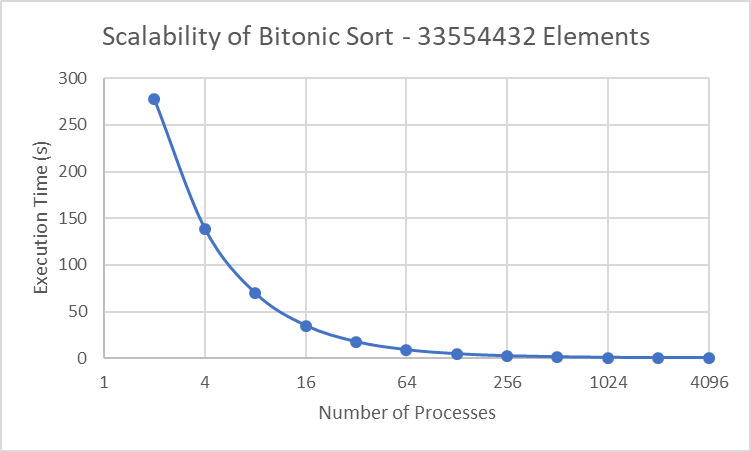
\includegraphics[scale=1]{bitonicsort_33554432_log}
\end{center}

Samplesort also showed speedup - to a certain extent - as the number of processes increased. It seems that there exists a happy medium between having a small enough array, but not too small to small to send too many messages across ranks. The ideal point seems to be at either 32 or 64 ranks. Beyond that number of ranks, communication between ranks slows down the execution time of the program. Under these number of ranks, the size of each array is large enough that traversal of the local array causes slowdown of the algorithm.

\begin{center}
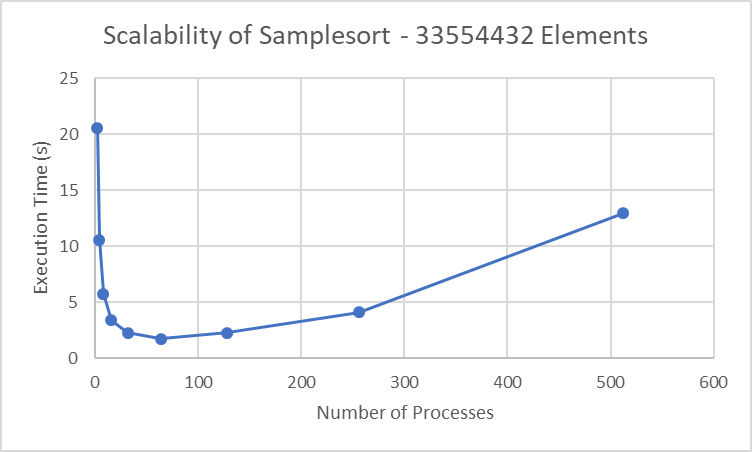
\includegraphics[scale=1]{samplesort_33554432}
\end{center}

However, what is most interesting about samplesort is how the algorithm scales with the number of elements. With a large number of processors, the execution time is quite large, but increases only slightly, compared to the doubling of the number of elements being sorted. Typically execution time at least doubles when the number of elements doubles. The following graphs depict the small increases in execution time of samplesort at 512 and 2048 processors and varying number of elements.

\begin{center}
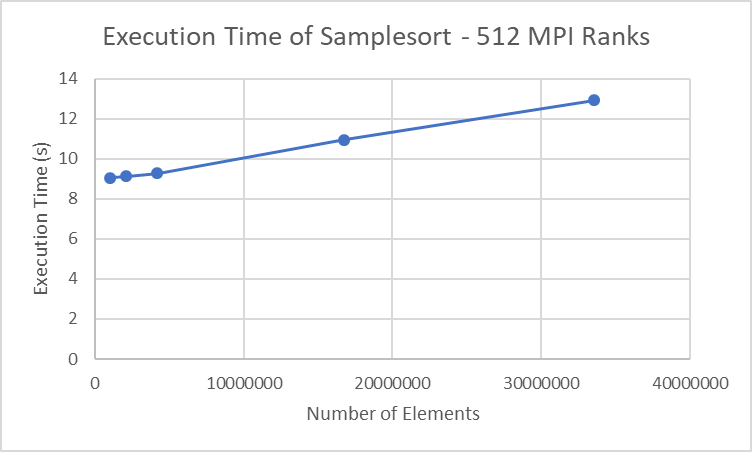
\includegraphics[scale=1]{samplesort_512}
\end{center}

\begin{center}
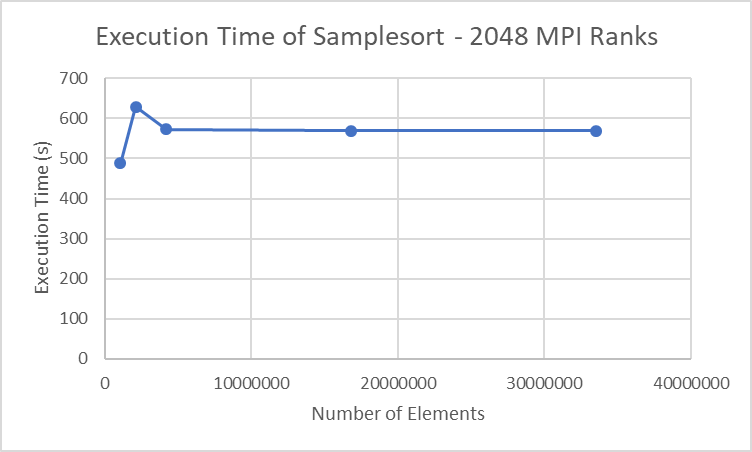
\includegraphics[scale=1]{samplesort_2048}
\end{center}

This is very different from the scalability of the other two algorithms as shown below. As the number of elements increases, the execution time increases similar to the theoretical limit asymptotic runtime of $O(n \log n)$.

\begin{center}
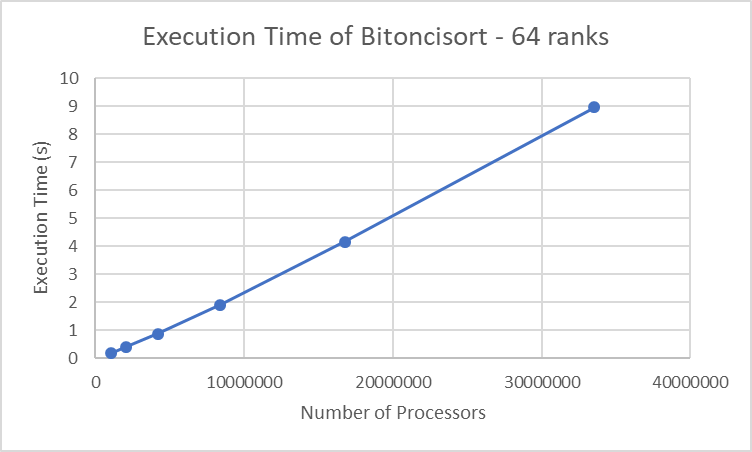
\includegraphics[scale=1]{bitonicsort_64}
\end{center}

At 512 ranks, There is a flat slope upwards in execution time as the number of elements significantly increases, as shown above. at 2048 ranks, the execution time is nearly completely flat, even as the number of elements doubles in size.

\begin{center}
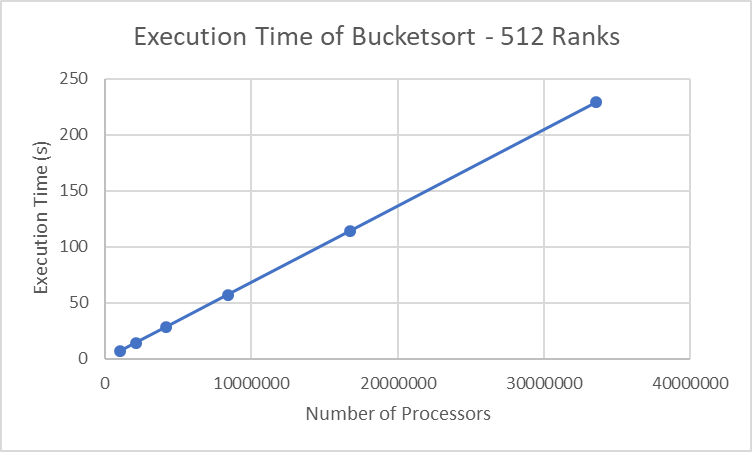
\includegraphics[scale=1]{bucketsort_512}
\end{center}

\section{Conclusion}
There is research here that can expand on in further analysis. As mentioned earlier, the current experiment only analyses performance of a list of randomly ordered integers. However, depending on the distribution or ordering of the elements in an array performance can be quite different. Future work could include analysis of the same algorithms with a nearly sorted list, a backwards sorted list, a Gaussian distribution, or a large number of repetitive elements. All of these environments could affect the runtime of each algorithm, and knowing more about the distribution of the input array may affect decisions about the ideal sorting algorithm to use.

Another opportunity for growth in this project may be to combine sorting algorithms together, based on their strengths, to create an effective and even more scalable large array sorting method. Depending on the situation, the program could determine a good quality sorting algorithm to use in that case, instead of using one sorting algorithm as a catch-all solution for all arrays. Another area to expand upon is how using threads to further increase parallelism as well as take advantage of shared memory to speed up sorting algorithms. In small core cases, using threads has been shown to speed up the execution time of parallel sorting algorithms \cite{DBLP:journals/corr/abs-1808-10292}. Taking advantage of threads may also help to make a more scalable sorting algorithm.

As is visible from the data, it is evident that parallel bitonic mergesort is an excellent choice when there are very many ranks available that can be devoted to sorting. When fewer ranks are available, Samplesort is a good option for a very large number of elements. Bucketsort shows promising scalability, but this implementation is much slower than the other sorts analyzed. Overall, parallel sorting algorithms are an important contribution to any high performance computing system, enabling users to quickly and efficiently sort very large arrays of numbers with available resources.


\bibliographystyle{acm}
\bibliography{bibliography}
\end{multicols}
\end{document}